\documentclass[a4paper, brazil, 12pt , onecolumn]{report}
\usepackage[T1]{fontenc}
\usepackage[utf8]{inputenc}
\usepackage[brazil]{babel}
\usepackage[dvips]{graphicx}
\usepackage{ae}
\usepackage[top=10mm,bottom=15mm,left=12mm,right=12mm]{geometry}
\usepackage{tabularx}
\usepackage{lipsum}
\usepackage{blindtext}
\usepackage{setspace}
\usepackage{color}
\usepackage{fancyhdr}
\usepackage{fancyvrb}
\usepackage{nomencl}
\usepackage{indentfirst}
\usepackage{amsmath}
\usepackage{listings}
\usepackage{subfigure}
\usepackage{xcolor} 
\definecolor{ocre}{RGB}{243,102,25} 
\usepackage{avant} 
\usepackage{mathptmx}
\usepackage{microtype}
\usepackage{makeidx}
\definecolor{almond}{rgb}{0.94, 0.87, 0.8}
\definecolor{blanchedalmond}{rgb}{1.0, 0.92, 0.8}
\usepackage[alf,abnt-etal-text=it,bibjustif, abnt-emphasize=bf, abnt-etal-list=0]{abntcite}
\newcommand{\ew}[1]               {\emph{#1}}
\newcommand{\ns}[1]               {\mbox{#1}}
\newcommand{\sigla}[1]            {\ns{#1}}
\newcommand{\italico}[1]          {\textit{#1}}
\newcommand{\negrito}[1]          {\textbf{#1}}
\newcommand{\subl}[1]             {\underline{#1}}
\newcommand{\cf}[1]               {\texttt{#1}}
\newcommand{\X}{\textbullet}
\newcommand{\Y}{$\circ$}
\renewcommand{\lstlistingname}{\bf Listagem} 

\definecolor{mygreen}{rgb}{0,0.6,0}
\definecolor{mygray}{rgb}{0.5,0.5,0.5}
\definecolor{mymauve}{rgb}{0.58,0,0.82}


\usepackage[Bjornstrup]{fncychap}
\title{Palestra \LaTeX}
\author{Luciano Senger}
\makeindex
\begin{document}
	\maketitle
	\tableofcontents
	\listoffigures
	\listoftables
\chapter{Redes Neurais}
Uma rede neural é um sistema computacional constituído de unidades de processamento simples, que tem a função de armazenar e tornar disponível para uso o conhecimento experimental~\cite{haykinredes, LeCun1990}.
A representação de um neurônio está ilustrada na Figura~\ref{fig:neuronio} e a ativação de um neurônio é descrita pela Equação~\ref{eq:ativacao}. 
\begin{equation}
	y_i = \sum_{i=0}^{n} w_i \times x_i
\end{equation}\label{eq:ativacao}

\begin{figure}[htb]
	\centering
	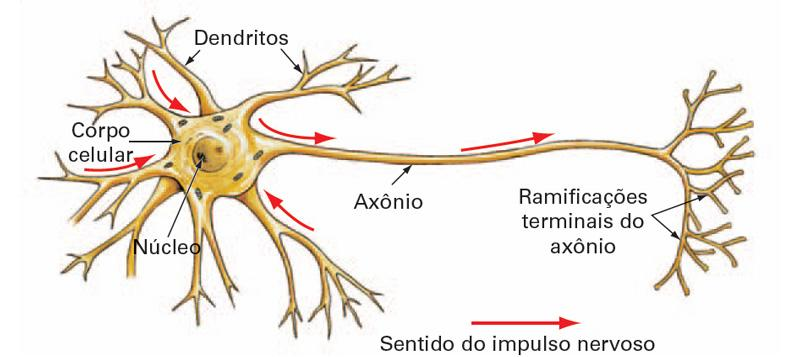
\includegraphics[scale=.3]{neuronio}
	\caption{Representação de um neurônio}\label{fig:neuronio}
\end{figure}
\chapter{Material e Métodos}\label{sec:mat}
\lipsum[3-8]
\lstset{language=Python}
\lstinputlisting[frame=single, numbers=left]{token.py}



\printindex
\appendix
\chapter{Análise estatística}
\lipsum[3-5]
\bibliographystyle{abnt-alf}
\bibliography{base}
\end{document}




